\section{习题课}
\subsection{基本概念}

1. 通信编码误差: $ \mathscr{E}=\{\mathscr{S}, \mathscr{C}\},(f, g) $ 固定, $ e(f, g)= $ $ \operatorname{Pr}\{\tilde{\xi} \neq \tilde{\eta}\} $ 为通信系统 $ \mathscr{E}(f, g) $ 所产生的编码误差.

2.几种类型的无记忆信道:

(1)无丢失信道: $ \xi $ 完全由 $ \eta $ 决定

(2)确定(决定)信道: $ \eta $ 完全由 $ \xi $ 决定

(3)无噪声信道: 无丢失且决定

(4)无用信道:由 $ \xi $ 得不到关于 $ \eta $ 的任何信息.

3. 信道矩阵

4.行对称、列对称、对称信道

5.信道容量: $ C=\max I(p(u) ; p(v \mid u)) $
\subsection{基本方法}

1. 利用定义计算二元对称信道, $ M $ 信道,四种典型无记忆信道的信道容量.

2. 利用极值法计算几种典型信道的信道容量(二元对称信道, $ M $ 信道,Z信道)

\subsection{课后习题}

\begin{exercise}
    写出二元对称信道,二元擦除信道及 $ M $ 信道的信道矩阵.
\end{exercise}
\begin{solution}
    \begin{figure}[h]
  \centering
  \begin{subfigure}[b]{0.3\textwidth}
    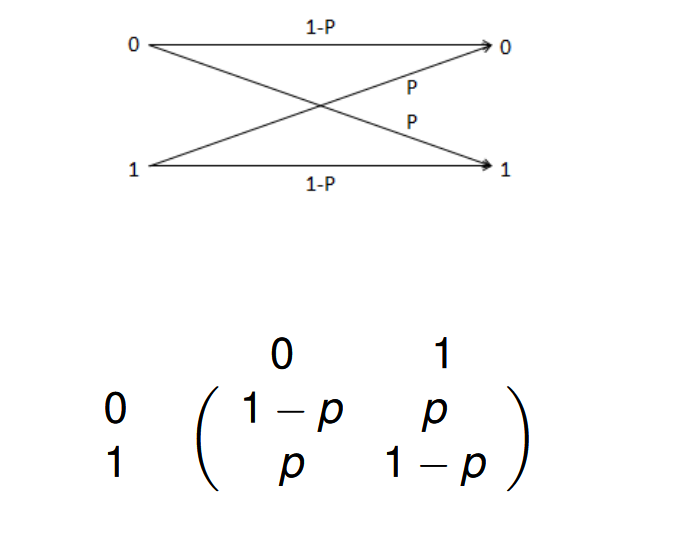
\includegraphics[width=\textwidth]{image/8.png}
    \caption{二元对称信道}
    \label{fig:image1}
  \end{subfigure}
  \hfill
  \begin{subfigure}[b]{0.3\textwidth}
    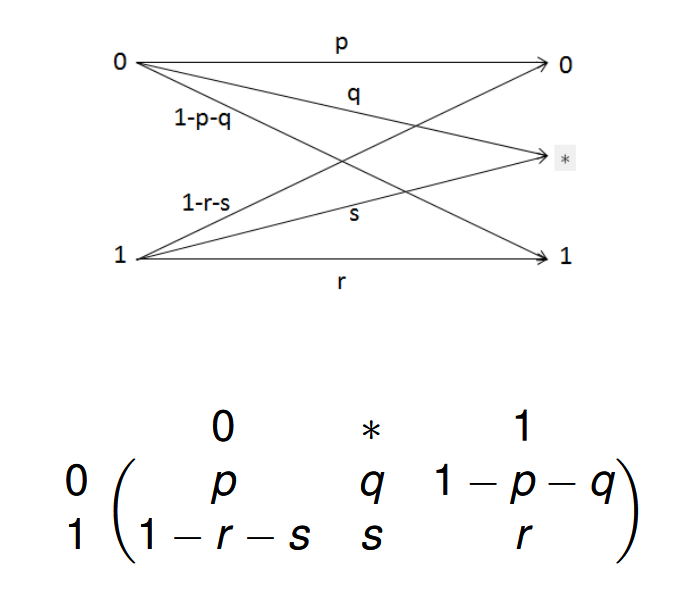
\includegraphics[width=\textwidth]{image/9.png}
    \caption{二元擦除信道}
    \label{fig:image2}
  \end{subfigure}
  \hfill
  \begin{subfigure}[b]{0.3\textwidth}
    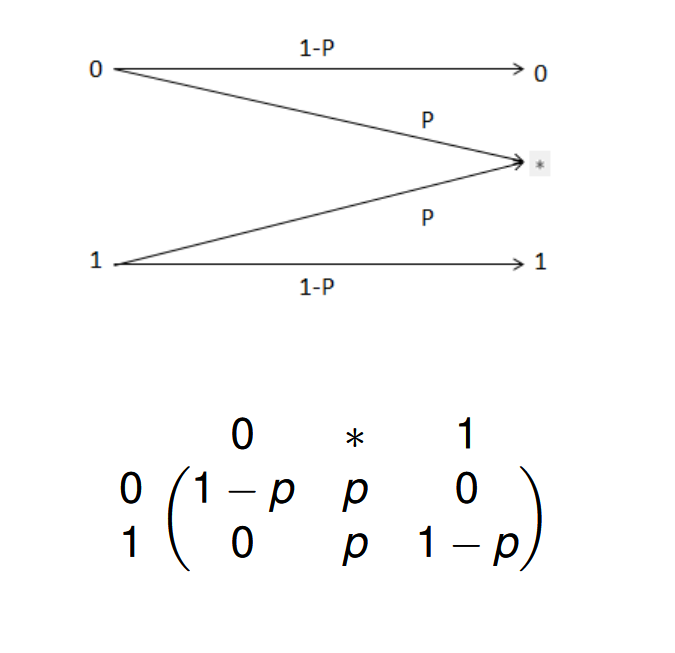
\includegraphics[width=\textwidth]{image/10.png}
    \caption{$ M $ 信道}
    \label{fig:image3}
  \end{subfigure}
  %\caption{}
  \label{fig:three_images}
\end{figure}
\end{solution}

\begin{exercise}
    Z信道如下图所示, 求其信道容量
    \begin{figure}[h]
        \centering
        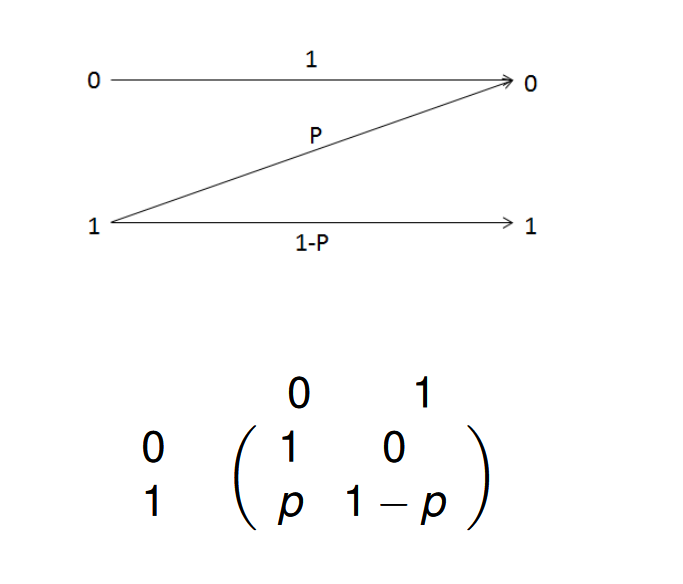
\includegraphics[width=0.4\linewidth]{image/11.png}
    \end{figure}
    \end{exercise}
    \begin{solution}
    根据信道容量的定义有$$C=p(0 \mid 0) \log \frac{p(0 \mid 0)}{q_{0}}+p(1 \mid 0) \log \frac{p(1 \mid 0)}{q_{1}}=p(0 \mid 1) \log \frac{p(0 \mid 1)}{q_{0}}+p(1 \mid 1) \log \frac{p(1 \mid 1)}{q_{1}}$$
$$
\begin{aligned}
\text{左边}&=\log \frac{1}{q_{0}}, \\
\text{右边}&=p \log \frac{p}{q_{0}}+(1-p) \log \frac{1-p}{q_{1}} \\
&=p \log p-p \log q_{0}+(1-p) \log (1-p)-(1-p) \log q_{1} \\
&=-H(p)-p \log q_{0}-(1-p) \log q_{1} .
\end{aligned}
$$
$$\left(q_{0}, q_{1}\right)=(\theta, 1-\theta)\left(\begin{array}{cc}1 & 0 \\ p & 1-p\end{array}\right)=(\theta+p(1-\theta),(1-\theta)(1-p))$$


$$ \begin{aligned}-\log q_{0}+p \log q_{0}+(1-p) \log q_{1}&=-H(p) \\ (1-p) \log q_{0}+(p-1) \log q_{1}&=H(p) \\ (1-p) \log \frac{q_{0}}{q_{1}}&=H(p)\\\log \frac{q_{0}}{q_{1}}&=\frac{H(p)}{1-p} \\ \frac{q_{0}}{q_{1}}&=2^{\frac{H(p)}{1-p}} \\ \frac{\theta+p(1+\theta)}{(1-\theta)(1-p)}&=2^{\frac{H(p)}{1-p}} \\ \frac{\theta-1+p(1-\theta)+1}{(1-\theta)(1-p)}&=2^{\frac{H(p)}{1-p}} \\ \frac{(1-\theta)(p-1)+1}{(1-\theta)(1-p)}&=2^{\frac{H(p)}{1-p}}\\-1+\frac{1}{(1-\theta)(1-p)}&=2^{\frac{H(\rho)}{1-p}} \\ \frac{1}{(1-\theta)(1-p)}&=2^{\frac{H(p)}{1-p}}+1 \\ \frac{1}{1-\theta}&=(1-p)\left[2^{\frac{H(p)}{1-p}}+1\right] \\ \theta&=\frac{1}{1-p}\left[-p+\frac{2^{\frac{H(p)}{1-p}}}{1+2^{\frac{H(p)}{1-p}}}\right]\end{aligned} $$
于是
$$ C=\log \frac{1}{\theta+p(1-\theta)}  =\log \frac{1}{\theta(1-p)+p}  =\log \frac{1+2^{\frac{H(p)}{1-p}}}{2^{\frac{H(p)}{1-p}}}=\log \left[1+2^{\frac{-H(p)}{1-p}}\right] . $$
    \end{solution}

\begin{exercise}
考虑离散无记忆信道 $ Y=(X+Z) \bmod 11 $, 其中
$$
Z=\left(\begin{array}{ccc}
1 & 2 & 3 \\
\frac1 3 & \frac1 3 & \frac1 3
\end{array}\right)
$$
$ X \in\{0,1, \cdots, 10\} $. 假设 $ X $ 和 $ Z $ 独立.\\
(1) 求这个信道的容量.\\
(2) 找出达到信道容量的入口分布.
\end{exercise}
\begin{solution}
(1) $ Y=(X+Z) \bmod 11 $, 输入为 $ X $, 输出为 $ Y, Z $ 为噪声信道, 而
$$
Z=\left(\begin{array}{ccc}
1 & 2 & 3 \\
\frac1 3 & \frac1 3 & \frac1  3
\end{array}\right), \quad X \in\{0,1, \cdots, 10\}
$$
所以 $ Y \in\{0,1, \cdots, 10\} $, 

因为 $ Z $ 可以取三个值 $ (1,2,3) $ ,每个都有 $ \frac{1}{3} $ 的概率,所以对于每个 $ X $ 的值, $ Y $ 可以是三个可能的结果之一,这取决于 $ Z $ 的值.信道矩阵 $ P(Y \mid X) $ 将具有 11 行 (对应于 $ X $ 的可能值) 和 11 列(对应于 $ Y $ 的可能值).每个元素 $ P_{i j} $ 表示给定输入 $ X=i $ 时输出 $ Y=j $ 的概率.

由于 $ Z $ 的作用是加在 $ X $ 上然后对 11 取模,每个 $ X $ 值将映射到三个不同的 $ Y $ 值,每个的概率都是 $ \frac{1}{3} $ .例如,如果 $ X=0 $ ,则 $ Y $ 可以是 $ 1 , 2 $ 或 3 ,每个都有 $ \frac{1}{3} $ 的概率,因为 $ Z $ 分别加 $ 1 , 2 $ 或 3 .因此,信道矩阵的一般形式将是每行有三个 $ \frac{1}{3} $ 的条目,分别对应于 $ X $ 加上 $ 1 , 2 , 3 $ 和模 11 的结果,而其他位置为 0 .对于 $ X=0: Y $ 的可能值是 $ 1,2,3 $ ,每个概率为 $ \frac{1}{3} $ . 对于 $ X=1: Y $ 的可能值是 $ 2,3,4 $ ,每个概率为 $ \frac{1}{3} $ .以此类推,直到 $ X=10 $ .每行的具体值会随着 $ X $ 的增加而“滚动”,并在达到 10 并绕回 0 时循环.这种模式的重复构成了完整的信道矩阵:

\begin{figure}[h]
    \centering
    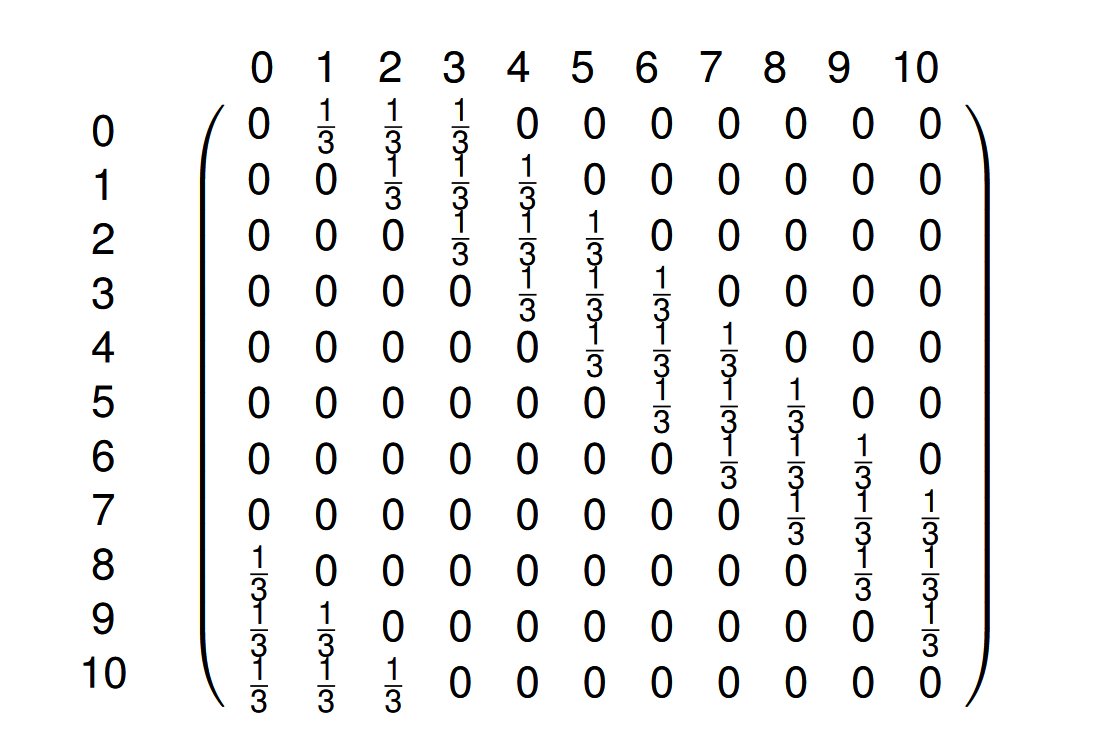
\includegraphics[width=0.6\linewidth]{image/12.png}
\end{figure}
可见 $ Z $ 对输入 $ X $ 的每个取值的作用效果一样, 这是一个对称信道, 因此
$$
\begin{aligned}
C & =\log 11-\left(\frac{1}{3} \log 3+\frac{1}{3} \log 3+\frac{1}{3} \log 3\right) \\
& =\log 11-\log 3=\log \frac{11}{3} .
\end{aligned}
$$

(2) 对于对称信道,最大化信道容量的输入分布是等概率分布. ,即
$$
p(X)=\frac{1}{11}, \quad, X \in\{0,1, \cdots, 10\} .
$$
\end{solution}

这个等概率分布的选择反映了信息论中的一个基本原则:当所有可能的事件(在这个情况下是输入信号的选择)都具有相同的概率时,不确定性(和因此信息熵)最大.在一个对称信道中,由于所有的输入对输出的影响是相同的,等概率分布确保了输出分布也尽可能均匀,从而最大化了从输入到输出的信息传递.
